\begin{figure}[H]
\begin{minipage}{.45\textwidth}

\centering
\resizebox{0.5\linewidth}{!}{%
    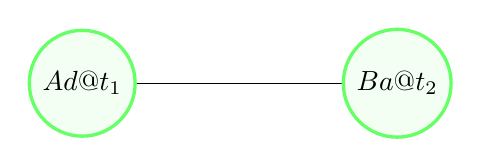
\begin{tikzpicture}[
roundnode/.style={circle, draw=green!60, fill=green!5, very thick, minimum size=8mm},
]
    
    \draw (0,0) -- (4,0);
    
    \draw (4,0) node[align=center,roundnode] {$Ba@t_2$};

    \draw (0,0) node[align=center,roundnode] {$Ad@t_1$};
    
    \end{tikzpicture}
%
}%
    \caption{An elementary connection betweens stations A and B, d stands for departure and a for arrival, $@t_i$ denotes the time the vehicle departs, arrives are waits (transfer)}
    \label{fig:transferel}

\end{minipage}\hspace{.1\textwidth}
\begin{minipage}{.45\textwidth}
\centering
\resizebox{0.5\linewidth}{!}{%
    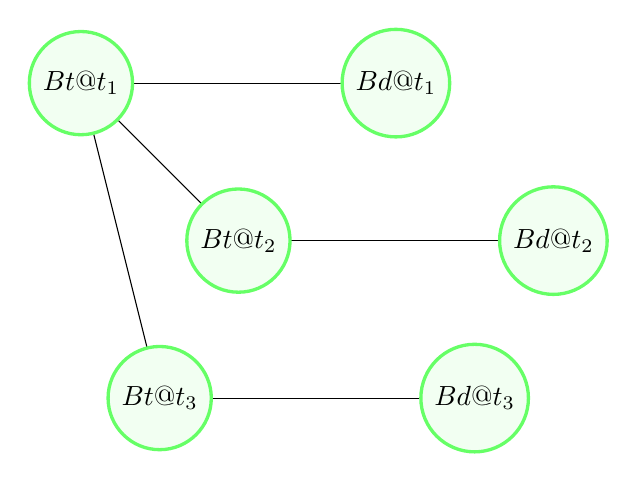
\begin{tikzpicture}[
roundnode/.style={circle, draw=green!60, fill=green!5, very thick, minimum size=8mm},
]
    
    \draw (0,0) -- (4,0);
    \draw (0,0) -- (2,-2);
    \draw (0,0) -- (1,-4);
    \draw (1,-4) -- (5,-4);
    \draw (2,-2) -- (6,-2);
    
    \draw (0,0) node[align=center,roundnode] {$Bt@t_1$};

    \draw (4,0) node[align=center,roundnode] {$Bd@t_1$};


    
    \draw (2,-2) node[align=center,roundnode] {$Bt@t_2$};

    \draw (6,-2) node[align=center,roundnode] {$Bd@t_2$};

    \draw (1,-4) node[align=center,roundnode] {$Bt@t_3$};

    \draw (5,-4) node[align=center,roundnode] {$Bd@t_3$};
    \end{tikzpicture}
%
}%
    \caption{An transfer, with an waiting chain}
    \label{fig:transferpatterntransfer}

\end{minipage}
\end{figure}